\section{Introduction}

Thermodynamics predates the atomic model and was created so that we can get the
most work out of machines for a given input. We began by studying bulk material
properties (think of a black box), however this is generalistic and it's
difficult to see the point. We can know a heat capacity, great. This doesn't
tell us anything about the physics that's going on, though.

In this course we will open the black box and look at the microscopic picture.
This really enriches our understanding, but we have to use statistical
mechanics. In a lecture hall, there are about $10^{30}$ atoms. With a 5Ghz
processor, this would take over the age of the universe to count (one per clock
cycle!) So what we really study is the average behaviour of many-bodied systems.

\section{Definitions}

Here we will use two systems to compare \emph{extensive} and \emph{intensive}
variables.
\begin{figure}[h!]
	\centering
	\includegraphics[width=0.8\textwidth]{IntensiveExtensiveVarComparison.png}
	\caption{Three systems that start all with the same initial conditions}
\end{figure}
\paragraph{Extensive variables} are ones which change when the system is split
up. For example:
\begin{itemize}
	\item Volume $V_A = 2V_B = 2V_C$
	\item Energy $U_A = 2U_B = 2U_C$
\end{itemize}

\paragraph{Intensive variables} are independent of the size of the system:
\begin{itemize}
	\item Temperature $T_A = T_B = T_C$
	\item Pressure $P_A = P_B = P_C$
\end{itemize}

\paragraph{The system} is the matter we're interested in.
\paragraph{The surroundings} is the rest of the universe.

\subsection{P-V Diagrams}

P-V diagrams are favourites in the thermodynamics community. They show the path
between two points of known pressure and volume:
\begin{figure}[h!]
	\centering
	\includegraphics[width=0.6\textwidth]{pVDiagramExample.png}
\end{figure}

\paragraph{Temperature} is a measure of how hot something is.
\paragraph{Heat} is energy in transit.

\section{Equations of state}

Equations of state describe a system mathematically:
$$
	f = f(p, V, T, \hdots)
$$
For example:
$$
	pV = RT \; \rightarrow \; f = f(p, V)
$$
Here we have two independent variables, and we can always find the third.

\section{Heat}

Heat always travels from a hot body to a cold body, if there is no external
influence.

\subsection{Heat capacity}

Heat capacity is a measure of how much energy is needed to increase the
temperature of a system:
$$
	C_v = \left(\frac{\partial Q}{\partial T}\right)_V
$$
We can then find the change in energy needed by integrating:
$$
	\Delta Q = \int^{T_2}_{T_1} C_v \cdot \mathrm{d} T
$$
There are two types of heat capacity that we use regularly. There is the heat
capacity at constant volume ($C_V$), and the heat capacity at constant pressure
($C_p$). The heat capacity at constant pressure is always higher because we need
to do work in increasing the volume of the gas, as well as the temperature.

\section{The Zero$^{th}$ Law of Thermodynamics}

This law is the basis of temperature. It says:
	
	If we have three systems, A, B and C, and we begin by letting A and B
	thermally equilibrate, then we have two systems in thermal equilibrium.
	If we then move B to C and there is no net heat transfer, meaning that B
	and C are already in equilibrium, then this means that A and C are in
	thermal equilibrium too - meaning they must be the same \emph{temperature}.

